\section{Classes}
\label{rear:classes}

This section will describe the concrete classes
building up \framework{}. Refer to figure \ref{fig:class_diagram}
for a more complete vision.

\subsection{The Robot Class}
\label{rear:classes:robotclass}

Let us have a look at the declaration of the \texttt{Robot}
class, reported in listing \ref{code:robot_class}.

\begin{lstlisting}[caption={\texttt{Robot} class declaration}, label={code:robot_class}, frame=trBL]
class Robot
{
 private:
  GLfloat x;
  GLfloat y;					
  GLfloat theta;

 public:
  Robot();
  GLfloat GetX();
  GLfloat GetY();
  GLfloat GetTheta();
  void Place(GLfloat x, GLfloat y, GLfloat theta);
  virtual void DrawRobot() = 0;
};
\end{lstlisting}

As already stated, private attributes of \texttt{Robot} 
are used to store the current position and orientation 
of the actual robot. Such attributes are initialized with 
all-zeros by the constructor, can be read by means 
of invoking their \textit{getter} methods and can be set 
by means of the \texttt{Place()} method.
\\
\texttt{Robot} also declares an abstract \textit{hook} method, 
\texttt{DrawRobot()}. Such a method is called by the 
\texttt{DataManager} every time it wants to render the 
robot model and, hence, programmers who wants to 
use \framework{} for their own robot should subclass 
\texttt{Robot} and implement \texttt{DrawRobot()} as a 
procedure that draws their custom robot model using 
the OpenGL API.
\\
When doing that, one must always keep in mind that 
\framework{} makes use of a three-dimensional OpenGL 
space, while position information is often represented 
as a \texttt{(x,y)} pair. \texttt{R.E.A.R.} maps the \texttt{x} 
value of such a pair onto the x axis of its OpenGL space, 
while the \texttt{y} value is mapped onto the z axis.
\\
That is, the actual XY plan corresponds to the OpenGL 
XZ plan. Such a correspondence is represented in figure 
\ref{fig:reference_systems}.

\begin{figure}[!h]
  \begin{center}
    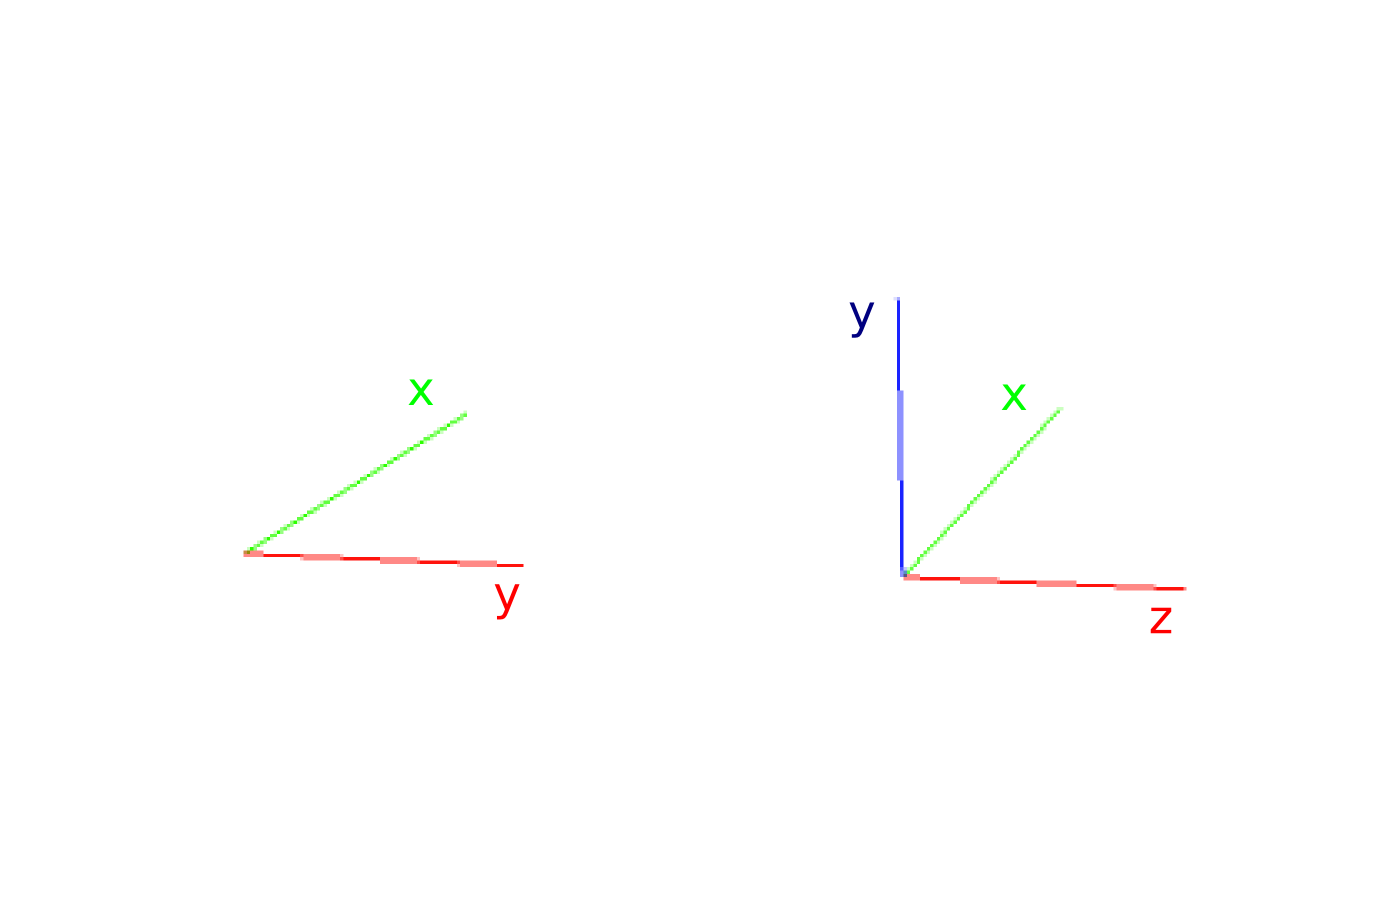
\includegraphics[width=300pt]{img/reference_system.png}
    \caption{Reference systems}
    \label{fig:reference_systems}
  \end{center}
\end{figure}

Moreover, to draw the robot in the right position within 
the OpenGL space, the first thing a \texttt{DrawRobot()} should 
do is to invoke OpenGL function \texttt{glTranslate()}.
\\
A skeleton of a concrete implementation of \texttt{DrawRobot()}
would look like this:
\begin{lstlisting}[caption={\texttt{DrawRobot()} skeleton}, label={code:drawrobot_skeleton}, frame=trBL]  
  glMatrixMode(GL_MODELVIEW);
  glPushMatrix();

  // set robot position
  glTranslatef(this -> x, 0.0f, this -> y);

  // rotate the robot 
  glRotatef(this -> theta, 0.0f, 1.0f, 0.0f);

  // code to actually draw the robot

  glPopMatrix();
\end{lstlisting}

\subsection{The Camera Class}
\label{rear:classes:cameraclass}

OpenGL does not provide any \textit{camera}, anyway it proved 
to be extremely useful to have a helper class that permits 
to easily set position and orientation of the user's 
point of view and sight, without worrying about lower-level 
OpenGL details.
\\
A basic implementation of such a helper class is suggested 
in \cite{opengl:camera}. Such an implementation is slightly 
similar the one featured by \framework{}, whose 
declaration is reported in listing \ref{code:camera_class}.

\begin{lstlisting}[caption={\texttt{Camera} class declaration}, label={code:camera_class}, frame=trBL]
class Camera
{
 private:
  SF3dVector Position;
  GLfloat RotatedX, RotatedY, RotatedZ;	
  GLfloat _theta;

 public:
  Camera();
  void Render ( void );
  void Move ( SF3dVector Direction );
  GLfloat GetX();
  GLfloat GetY();
  GLfloat GetZ();
  GLfloat GetTheta();
  void SetPosition(GLfloat x, GLfloat y, GLfloat z);
  void SetYAngle ( GLfloat Angle );
  void RotateX ( GLfloat Angle );
  void RotateY ( GLfloat Angle );
  void RotateZ ( GLfloat Angle );
  void RotateXYZ ( SF3dVector Angles );
};
\end{lstlisting}

The \texttt{Camera} class allows to move and rotate the user 
point of view, independently from the robot.
\\
This is essential for our purposes, since \framework{}
must be able to draw the robot everywhere in the OpenGL space, 
regardless of where the camera is, and vice versa.
\\
\texttt{Camera} methods are pretty simple: they just make 
use of OpenGL basic commands (such as \texttt{glTranslate} 
and \texttt{glRotate}) to actually move the OpenGL reference 
system and, hence, move the point-of-view and change the sight 
direction.
\\
The only thing to care about when using such a class is 
to invoke the OpenGL commands \texttt{glMatrixMode(GL\_MODELVIEW)} 
and \texttt{glLoadIdentity()} before invoking its 
\texttt{Render()} method. This avoids previous modifications 
of the \texttt{GL\_MODELVIEW} matrix from affecting the 
positioning of the camera.


\subsection{The DataManager Class}
\label{rear:classes:datamanager}

As already stated, the \texttt{DataManager} class is the \textit{core}
of the whole framework. Its declaration is reported in 
listing \ref{code:datamanager_class}.

\begin{lstlisting}[caption={\texttt{DataManager} class declaration}, label={code:datamanager_class}, frame=trBL]
class DataManager
{
 private:
  GLuint _texture[1];
  Robot * _rob;
  Camera * _camera;
  IDataLogic * _logic;
  IImageSelector * _calculator;

  robot_data * _robot_status;
  image_data * _bg_image_data;

  /* bind the specified image to a texture */
  void LoadGLTextures(GLuint *, const char *);

 public:
  DataManager(Robot *, DataLogic *, Camera *, 
	      IImageSelector *); 
  ~DataManager();
  void NextStep(int command = 0);
};
\end{lstlisting}

Of course, \texttt{DataManger} is meant to be used as a \textit{singleton}, 
that is, there must be a unique instance of \texttt{DataManager} 
within the context of a \framework{} based application.
\\
As its name suggests, \texttt{DataManager} manages and coordinates 
all of the components of the exocentric vision system and, hence, 
keeps a private reference to all of them: 
the \texttt{Robot} instance (see section \ref{rear:classes:robotclass}), the 
\texttt{Camera} instance (see section \ref{rear:classes:cameraclass}),
a \texttt{IDataLogic} object, a \texttt{IImageSelector} 
object and an OpenGL texture id number.
\\
Once the application is started, it's \texttt{DataManger}'s duty 
to move robot and camera within the OpenGL space. Moreover, 
it's also responsible for 1. providing the user an interface 
to send commands to the robot, 2. retrieving position 
data from the actual robot every time the user asks 
for it, 3. for picking one of the available snapshots, 
4. displaying it in the background. 
\\
All of these operations are performed within the 
scope of \texttt{NextStep()} method, reported in 
listing \ref{code:next_step}.

\begin{lstlisting}[caption={The \texttt{DataManager::NextStep()} method}, label={code:next_step}, frame=trBL]
void DataManager::NextStep(int command) {

  image_data old_image;

  // save metadata of the currently displayed 
  // image
  old_image.x = _bg_image_data -> x;
  old_image.y = _bg_image_data -> y;
  old_image.theta = _bg_image_data -> theta;


  // send command to the robot
  _logic->Command(command);

  // retrieve new data from the robot
  _logic->RetrieveData(_robot_status);

  // move robot with _robot_status data
  _rob->Place(_robot_status->x,
	      _robot_status->y,
	      _robot_status->theta ); 

  // choose an image to set as background
  _logic->SelectImage(_robot_status, _bg_image_data,
		      _calculator);

  // if the chosen image is not the currently
  // displayed one, then  move the camera
  // into the new position and change its 
  // orientation accorgindly
  if ( old_image.x != _bg_image_data -> x ||
       old_image.y != _bg_image_data -> y ||
       old_image.theta != _bg_image_data -> theta )
    {
      _camera -> SetPosition( _bg_image_data -> x,
			      0.f,
			      _bg_image_data -> y);
      
      _camera -> SetYAngle( _bg_image_data -> theta - 90);
    }

  // actually set the chosen image as background
  LoadGLTextures(_texture, _bg_image_data->path);
}
\end{lstlisting}

\texttt{NextStep()} has to be called every time 
the user wants to send a command to the robot.
Such a command, encoded as an integer, has to be passed to 
\texttt{NextStep()} as an argument.
\\
Then, \texttt{DataManager} asks its \texttt{IDataLogic} 
instance to send the command to the robot and to 
retrieve the new robot position and orientation, which will be 
stored in the \texttt{\_robot\_status} private attribute.
\\
To select an image to set as background, \texttt{DataManager} 
invokes the \\
\texttt{IDataLogic::SelectImage()} method, 
passing it the current robot position and orientation, 
an object of type \texttt{IImageSelector} which 
encapsulates the image selection algorithm and a structure 
of type \texttt{image\_data}.
\\
The method will fill the fields of such a structure with 
the metadata of the selected image, so that the 
\texttt{DataManager()} can pick it up, load it as a 
texture and display it on the background of the 
viewing frustum - by means of calling the 
\texttt{LoadGLTextures()} function.
\\
In order to give the illusion of watching the scene 
from the point the selected image was taken, 
\texttt{NextStep()} also moves the camera and change 
its orientation accordingly to the image metadata.
